
Developers often have to deal with conflicting goals that require software to be delivered quickly, with high quality, and on budget. In practice, achieving all of these goals at the same time can be challenging, causing a tradeoff to be made. Often, these tradeoffs lead developers to take \emph{shortcuts} or use \emph{workarounds}. Although such shortcuts help developers in meeting their short-term goals, they may have a negative impact in the long-term.

Technical debt is a metaphor that has been used to express sub-optimal solutions that are taken consciously in a software project in order to achieve some short-term goals. Generally, these decisions allow the project to move faster in the short-term, but introduce an increased cost (i.e., debt) to maintain this software in the long run~\cite{Seaman2011,Kruchten2013IWMTD}. Prior work showed that technical debt is widespread in the software domain, is unavoidable, and can have a negative impact on the quality of the software~\cite{Lim2012Software}.

Due to the importance of technical debt, a number of studies empirically examined it and proposed techniques to enable its detection and management. The main findings of the prior work is that 1) there are different types of technical debt, e.g., defect debt, design debt, testing debt, and that design debt has the highest impact~\cite{Alves2014MTD,Marinescu2012IBM}; and 2) statically analyzing the source code can help detecting technical debt~\cite{Marinescu2004ICSM,Marinescu2010CSMR,Zazworka2013CSE}. In particular, these works use metric thresholds to detect code smells, which are considered as proxies for technical debt. 

One major drawback of using metrics to detect technical debt is that no one knows if the detected smells really constitute technical debt, or if they correspond to problems that the developers care about. Therefore, more recently, our work showed that using code comments can be effective in identifying self-admitted technical debt~\cite{Potdar2014ICSME}. This work uses comments to detect \emph{generic} technical debt, and did not focus on any specific type of technical debt.


\begin{figure*}[thb!]
    \centering
    \label{fig:approach}
    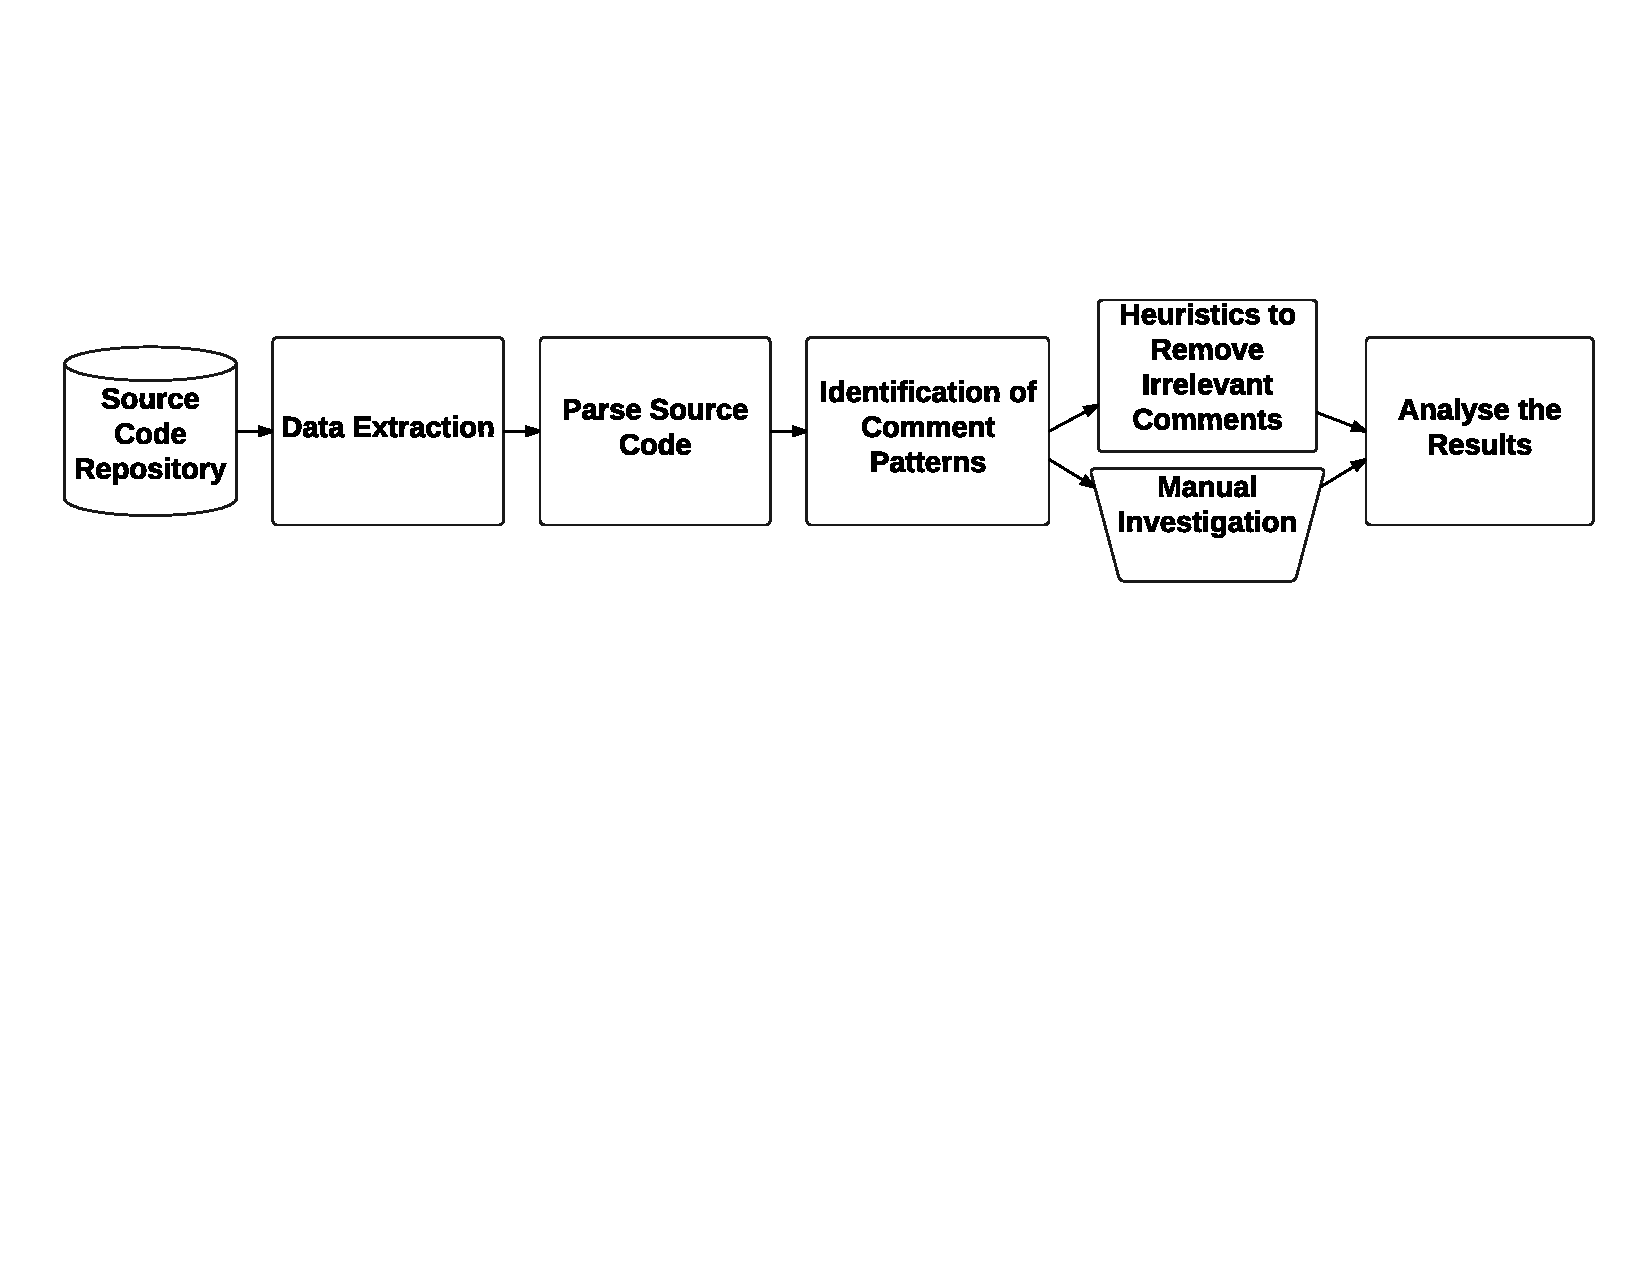
\includegraphics[width=1\textwidth]{figures/Approach2}
    %Caption goes below the figure
    \vspace{-10mm}
    \caption{Approach overview}
\end{figure*}


In this paper, we build on the promising approach of using code comments to detect one of the most impacting types of debt, namely \emph{design technical debt}, which we call \SADTD. We manually examine more than 17,000 code comments to extract comment patterns that can be used to detect \SADTD. To examine the effectiveness of our approach, we perform an empirical study on ten open source projects. Finally, we compare our approach to state-of-the-art approaches and examine the effectiveness of using automated refactoring techniques in mitigating \SADTD.

Based on our manual examination of the code comments, we derive 176 different comment patterns that can be used to detect \SADTD. These patterns are able to detect \SADTD with a precision ranging in 74.0-96.30\% and a recall ranging in 10.87-83.87\%. Moreover, we find that the design technical debt found with our approach is different than the design technical debt found using metric-based approaches~\cite{Zazworka2013CSE}. Finally, we find that automated refactoring can address up to 24.58\% of the methods containing \SADTD.

The rest of the paper is organized as follows:  Section~\ref{sec:motivating_example} presents a motivating example. Section~\ref{sec:approach} details our approach. We present our case study results in Section~\ref{sec:case_study_results}, followed by a discussion in Section \ref{sec:discussion}. Section~\ref{sec:related_work} presents the related work. The threats to validity of our work are discussed in Section~\ref{sec:threats_to_validity}. Section~\ref{sec:conclusion} lists the conclusions of our work.